% LaTeX document class and packages
\documentclass[journal]{IEEEtran}
\usepackage[a5paper, margin=10mm, onecolumn]{geometry}
\usepackage{tfrupee}
\usepackage{gvv-book}
\usepackage{gvv}
\usepackage{cite}
\usepackage{amsmath,amssymb,amsfonts,amsthm}
\usepackage{algorithmic}
\usepackage{graphicx}
\usepackage{textcomp}
\usepackage{xcolor}
\usepackage{txfonts}
\usepackage{listings}
\usepackage{enumitem}
\usepackage{mathtools}
\usepackage{gensymb}
\usepackage{comment}
\usepackage[breaklinks=true]{hyperref}
\usepackage{tkz-euclide}
\usepackage{listings}
\usepackage[latin1]{inputenc}
\usepackage{color}
\usepackage{array}
\usepackage{longtable}
\usepackage{calc}
\usepackage{multirow}
\usepackage{hhline}
\usepackage{ifthen}
\usepackage{lscape}
\usepackage{circuitikz}
\usepackage{float}
\usetikzlibrary{patterns}
\renewcommand{\thefigure}{\theenumi}
\renewcommand{\thetable}{\theenumi}
\setlength{\intextsep}{10pt}
\numberwithin{equation}{enumi}
\numberwithin{figure}{enumi}

\begin{document}
\bibliographystyle{IEEEtran}
\vspace{3cm}

\title{CE\\2012}
\author{EE24BTECH11063 - Y.Harsha Vardhan Reddy}
\maketitle

\bigskip

\section*{Q.10 to Q.22 carry 2 marks each}
\begin{enumerate}
    \item A uniform flow with a velocity of 2 m/s in the x-direction approaches a line source placed on the x-axis at a distance of 0.1 m from the origin. If the origin is the stagnation point in the resulting flow, the strength of the source (in m$^2$/s, rounded off to 2 decimal places) is \underline{\hspace{1cm}}.
\bigskip

\item In a steady incompressible flow of a fluid past a smooth stationary sphere, the drag force $F$ depends on the flow velocity $U$, diameter $D$, and the dynamic viscosity $\mu$ and density $\rho$ of the fluid. Experiments are conducted on the same sphere at the same flow velocity using two different fluids. The density of the second fluid is two times that of the first fluid. The dynamic viscosity of the second fluid is $n$ times that of the first fluid. If the non-dimensional force $F / (\rho U^2 D^2)$ remains the same in both the experiments, the value of $n$ is \underline{\hspace{1cm}}.
\bigskip

\item An incompressible fluid flows past a flat plate as shown in the figure below$\ref{fig:1}$ with a uniform inlet velocity profile $u = U$ and a parabolic exit velocity profile $u = U(2\eta - \eta^2)$, where $u$ is the component of velocity parallel to the wall, $y$ is the normal distance from the plate, and $\eta = y / \delta$. If the volume flow rate across the top surface of the control volume (CV) is $Q = p U \delta$ per unit width (perpendicular to the x-y plane) of the plate, the value of $p$ (rounded off to 2 decimal places) is \underline{\hspace{1cm}}.
\begin{figure}[H]
    \centering
    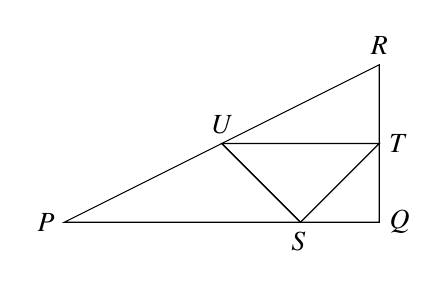
\begin{tikzpicture}
\draw (0,0) node[left] {$P$} -- (4,0) node[right] {$Q$} -- (4,2) node[above] {$R$} -- cycle;
\draw (3,0) node[below] {$S$} -- (2,1) node[above] {$U$} -- (4,1) node[right] {$T$} -- cycle;
\draw (2,1) -- (3,0);
\end{tikzpicture}

    \caption{}
    \label{fig:1}
\end{figure}
\bigskip

\item A jet engine is to be tested on a thrust stand as shown in the figure below$\ref{fig:2}$. The conditions prevailing in typical test are as follows: Axial intake air velocity=100 m/s; axial exhaust gas velocity=250m/s; intake cross-sectional area =$1\;m^2$; intake static pressure=$-22\;kPa$(gauge); exhaust static pressure = $0\;\text{kPa}$(gauge); mass flow rate throgh the engine = 100kg/s. The anchoring force (in kN) in axial direction on the thrust stand is \underline{\hspace{1cm}}
\begin{figure}[H]
    \centering
    \scalebox{0.5}{
\begin{circuitikz}
\tikzstyle{every node}=[font=\normalsize]
\draw (4.25,10) to[short] (11,10);
\draw (4.25,7.75) to[short] (6.75,7.75);
\draw (8.5,7.75) to[short] (11,7.75);
\draw (6.75,5.25) to[short] (6.75,7.75);
\draw (8.5,5.25) to[short] (8.5,7.75);
\draw [dashed] (6,6.75) -- (9.25,6.75)node[pos=0.9,above, fill=white]{R};
\draw [->, >=Stealth] (7.5,7.25) -- (7.5,6)node[pos=0.85,below, fill=white]{V=?};
\draw [->, >=Stealth] (9.25,6) -- (8.5,6.5);
\draw [short] (9.25,6) -- (11,6)node[pos=1, fill=white]{dia = 2 m};
\draw [dashed] (10,7.25) -- (10,10.5)node[pos=0.95,right, fill=white]{Q};
\draw [dashed] (5,7.25) -- (5,10.5)node[pos=0.95,left, fill=white]{P};
\draw [->, >=Stealth] (3.75,9) -- (5.75,9)node[pos=0, fill=white]{V=6m/s};
\draw [->, >=Stealth] (8.75,9) -- (10.75,9)node[pos=0.95,right, fill=white]{V=5m/s};
\draw [->, >=Stealth] (6.25,10.5) -- (6,9.5);
\draw [->, >=Stealth] (8.75,10.5) -- (9,9.5);
\draw [short] (8.25,10.5) -- (8.75,10.5)node[pos=0,left, fill=white]{dia = 4m};
\draw (6.25,10.5) to[short] (6.75,10.5);
\end{circuitikz}
}

    \caption{}
    \label{fig:2}
\end{figure}
\bigskip
\end{enumerate}
\begin{enumerate}
\section*{Q.1 to Q.9 carry 1 mark each}
\item On decreasing the objective aperture size in an optical microscope

\begin{enumerate}
    \item the spherical aberration increases
    \item the depth of field increases
    \item the diffraction-limited resolution increases
    \item the astigmatism increases
\end{enumerate}
\bigskip

\item Pilling-Bedworth ratios for oxides of some metals are given in the table.

\begin{table}[h]    
  \centering
  \begin{tabular}[12pt]{ |c| c|}
    \hline
    \textbf{Variable} & \textbf{Description}\\ 
    \hline
    $V_1,u_1,f_1$ & Parameters of Parabola \\
    \hline 
    $V_2,u_2,f_2$ & Parameters of circle \\
    \hline
     $P_1,P_2$ & Points of intersection \\
     \hline
     $A$ & Area between the conics \\
    \hline
\end{tabular}

\end{table}

Based on the criterion of Pilling-Bedworth ratio alone, which one of the following metals will be most protected from high temperature oxidation?

\begin{enumerate}
\begin{multicols}{4}
    \item Li
    \item Ce
    \item Ta
    \item W
    \end{multicols}
\end{enumerate}
\bigskip

\item In NaCl, the substitution of a Na$^+$ ion by a Ca$^{2+}$ ion would most probably lead to

\begin{enumerate}
    \item the formation of a Na$^+$ vacancy
    \item the creation of a Cl$^-$ interstitial
    \item the formation of a Cl$^-$ vacancy
    \item the formation of a Na$^+$ and Cl$^-$ vacancy pair
\end{enumerate}
\bigskip

\item Which one of the following is time-independent?

\begin{enumerate}
\begin{multicols}{2}
    \item Elastic deformation
    \columnbreak
    \item Anelastic deformation
    \end{multicols}
    \begin{multicols}{2}
    \item Viscoelastic deformation
    \item Creep deformation
\end{multicols}
\end{enumerate}
\bigskip

\item Copper is diffused into aluminium at 400 $^{\circ}$C for 100 hours to obtain a certain concentration at a given depth. In another experiment conducted at 500 $^{\circ}$C, to achieve the same concentration of copper at the same depth, the time required in hours is

(Given: Diffusion coefficients of copper in aluminium at 400 $^{\circ}$C and 500 $^{\circ}$C are 5 $\times$ 10$^{-14}$ m$^2$ s$^{-1}$ and 6 $\times$ 10$^{-13}$ m$^2$ s$^{-1}$, respectively)

\begin{enumerate}
\begin{multicols}{4}
    \item 7.33
    \item 8.33
    \item 9.33
    \item 10.33
    \end{multicols}
\end{enumerate}

\item If carbon (C) in iron (Fe) is 6 percent by weight, then its atomic percent is approximately

(Given: atomic weight C = 12, Fe = 56)

\begin{enumerate}
\begin{multicols}{4}
    \item 13
    \item 23
    \item 30
    \item 50
    \end{multicols}
\end{enumerate}
\bigskip

\item GaAs has advantage over silicon when used in integrated circuits at low power because it has

\begin{enumerate}
    \item larger band gap
    \item more than one element
    \item higher electron mobility
    \item higher hole mobility
\end{enumerate}
\bigskip

\item Glass transition temperature of a polymer can be determined by

\begin{enumerate}
    \item Thermo-gravimetric analysis
    \item Raman spectroscopy
    \item NMR spectroscopy
    \item Differential scanning calorimetry
\end{enumerate}
\bigskip

\item The maximum wavelength of radiation to which Germanium (Ge) is opaque will be

(Given: energy gap of Ge = 0.67 eV, Planck's constant $h = 6.63 \times 10^{-34}$ J$\cdot$s, velocity of light $c = 3 \times 10^8$ m s$^{-1}$, and $1$ eV $= 1.6 \times 10^{-19}$ J)

\begin{enumerate}
\begin{multicols}{4}
    \item 0.8 $\mu$m
    \item 1.8 $\mu$m
    \item 2.8 $\mu$m
    \item 4.8 $\mu$m
    \end{multicols}
\end{enumerate}
\end{enumerate}

\end{document}
    
